\documentclass{standalone}
\usepackage{amsmath, amssymb, amsthm}
\usepackage{tikz}

\usetikzlibrary{shapes.geometric, arrows}
\newcommand{\ENC}{\text{ENC}}

\tikzstyle{txt} = [fill=white, rectangle,
    minimum width=0.5cm, minimum height=0.5cm]
\tikzstyle{block} = [draw, fill=white, rectangle, 
    minimum width=1cm, minimum height=0.5cm]
\tikzstyle{arrow} = [thick, ->, >=stealth]
\tikzstyle{oplus} = [fill=white, circle]
\begin{document}
    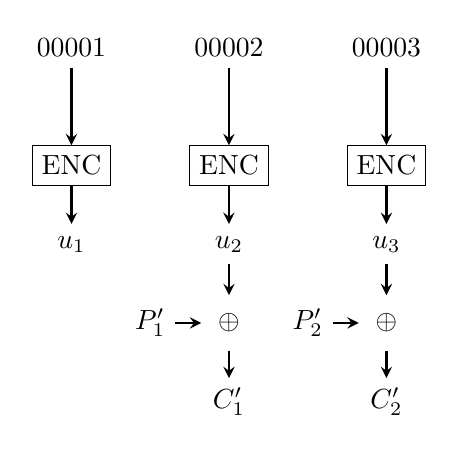
\begin{tikzpicture}[node distance=1.5cm]
        \node [txt] (i0) at (0, 0) {$00001$};
        \node [txt] (i1) at (2, 0) {$00002$};
        \node [txt] (i2) at (4, 0) {$00003$};
        %\node [txt] (i3) at (6, 0) {$00003$};

        \node [block, below of=i0] (e0) {$\ENC$};
        \node [block, below of=i1] (e1) {$\ENC$};
        \node [block, below of=i2] (e2) {$\ENC$};
        %\node [block, below of=i3] (e3) {$\ENC$};

        \node [txt, below of=e0, node distance=1cm] (u0) {$u_1$};
        \node [txt, below of=e1, node distance=1cm] (u1) {$u_2$};
        \node [txt, below of=e2, node distance=1cm] (u2) {$u_3$};
        %\node [txt, below of=e3, node distance=1cm] (u3) {$u_3$};

        \node [oplus, below of=u1, node distance=1cm] (x1) {$\oplus$};
        \node [oplus, below of=u2, node distance=1cm] (x2) {$\oplus$};
        %\node [oplus, below of=u3, node distance=1cm] (x3) {$\oplus$};
        
        \node [txt, left of=x1, node distance=1cm] (p1) {$P'_1$};
        \node [txt, left of=x2, node distance=1cm] (p2) {$P'_2$};
        %\node [txt, left of=x3, node distance=1cm] (p3) {$P_3$};

        \node [txt, below of=x1, node distance=1cm] (c1) {$C'_1$};
        \node [txt, below of=x2, node distance=1cm] (c2) {$C'_2$};
        %\node [txt, below of=x3, node distance=1cm] (c3) {$C_3$};

        \draw [arrow] (i0) -- (e0); \draw [arrow] (e0) -- (u0);
        \draw [arrow] (i1) -- (e1); \draw [arrow] (e1) -- (u1); \draw [arrow] (u1) -- (x1); \draw [arrow] (p1) -- (x1); \draw [arrow] (x1) -- (c1);
        \draw [arrow] (i2) -- (e2); \draw [arrow] (e2) -- (u2); \draw [arrow] (u2) -- (x2); \draw [arrow] (p2) -- (x2); \draw [arrow] (x2) -- (c2);
        %\draw [arrow] (i3) -- (e3); \draw [arrow] (e3) -- (u3); \draw [arrow] (u3) -- (x3);; \draw [arrow] (p3) -- (x3); \draw [arrow] (x3) -- (c3);
    \end{tikzpicture}

\end{document}